% 報告会テンプレート(LuaLaTeX対応版)
\documentclass[10pt,a4j,twocolumn]{ltjsarticle}


\usepackage{graphicx}   % \includegraphics を使うためのパッケージ読み込み
\usepackage{imcreport}  % IMC報告会用テンプレートパッケージの読み込み

\usepackage{newtxmath}
\usepackage{amsmath,amssymb}
\usepackage{bm}

% ハイフネーションを抑制する。数値が大きいほど、無理にでも抑制しようとする。
\hyphenpenalty=10000\relax
\exhyphenpenalty=10000\relax
\sloppy


\title{動的マニピュレータに対する不確実性分散の拡張についての検討} % タイトル
\author{高谷秀明}                              % 著者
\studentnumber{TD18K001}                         % 学籍番号
\date{2019--04--18}                              % 日付
\header{中間報告}                                % 左上のヘッダ内容


\begin{document}

\maketitle

\section{はじめに}

マニピュレータがアーム長さのようなパラメータに不確かさを持つ場合、不確かさは手先へと伝播し、その結果手先位置も不確かさを持つようになる。
先行研究では手先位置の確率分布の大きさを表す評価関数として不確実性分散(UV)を設計し、この評価関数を用いてマニピュレータの不確かさ解析や姿勢最適化を行った。

しかしUVは静的マニピュレータに対して定義した評価関数であるため、動的マニピュレータには適用することができないという問題を持つ。
この問題を解決するアプローチとして、(A)~動的マニピュレータに対応する既存の評価関数に不確実性分散の性質を取り入れる、(B)~不確実性分散を動的マニピュレータへ拡張する、などが考えられる。

本報告書では、アプローチ(A)として吉川が提案した可操作度に不確かさの影響を取り入れる方法を提案する。
可操作度は簡単な式変形で動的可操作度に拡張することが可能であるため、不確かさを取り入れた可操作度が有効であれば動的マニピュレータへの拡張も可能であると考えられる。
手法の提案に加えて、本報告書では2リンクマニピュレータに手法を適用した結果を示す。

\section{静的マニピュレータと可操作度}

静的マニピュレータは姿勢$\bm{q} \in \mathbb{R}^{m}$から手先位置$\bm{r} \in \mathbb{R}^{n}$を求める関数$\bm{f}$としてモデル化される。
\begin{equation}
  \bm{r} = \bm{f}(\bm{q}). \label{eq:static_manipulator_position}
\end{equation}
式~\eqref{eq:static_manipulator_position}の両辺を時刻$t$で微分すると、
%式~\eqref{eq:static_manipulator_position}の両辺を時刻$t$で微分すると速度についてのモデルが得られる。
\begin{equation}
  \dot{\bm{r}} = \bm{J}(\bm{q}) \dot{\bm{q}}. \label{eq:static_manipulator_velocity}
\end{equation}
ここで$\bm{J} = [\partial f_{i} / \partial q_{j}]_{1 \leq i \leq m, 1 \leq j \leq n}$はマニピュレータのヤコビアンである。

式~\eqref{eq:static_manipulator_velocity}のマニピュレータに対する可操作度$M$は次式で与えられる。
\begin{equation}
  M(\bm{q}) = \sqrt{\det \left( \bm{J}(\bm{q}) \bm{J}^{\mathrm{T}}(\bm{q}) \right)}.
\end{equation}
指標$M$は姿勢$\bm{q}$の変化に対する$\bm{r}$の変化の大きさを表す。
可操作度が大きいことはマニピュレータの運動性能が高いことを意味する。

\section{不確かさを取り入れた可操作度}

マニピュレータが確率変数を$\bm{\xi} \in \mathbb{R}^{l}$で表される不確かさを持つ場合、式~\eqref{eq:static_manipulator_velocity}は次式で書き換えられる。
\begin{equation}
  \dot{\bm{r}} = \bm{J}^{*}(\bm{q}, \bm{\xi}) \dot{\bm{q}}. \label{eq:static_manipulator_velocity_with_uncertainty}
\end{equation}
ここで$\bm{J}^{*}$は不確かさもモデル化したヤコビアンである。

このときの可操作度は、
\begin{equation}
  M(\bm{q}, \bm{\xi}) = \sqrt{\det \left( \bm{J}^{*}(\bm{q}, \bm{\xi}) \bm{J}^{*\mathrm{T}}(\bm{q}, \bm{\xi}) \right)}.
\end{equation}
以下ではこの$M$を拡張可操作度と呼ぶことにする。
本研究では$M$の統計量から不確かさが手先運動に与える影響を推定できるという仮説を立てた。
次節ではこのことをシミュレーションで検証する。

\section{拡張可操作度の検証}

2リンクマニピュレータに対して、(I)アームの長さに不確かさがある場合、(II)リンク角度に不確かさがある場合、について計算した拡張可操作度を図~\ref{fig:case_i}~,\ref{fig:case_ii}に示す。
\begin{figure}
  \centering
  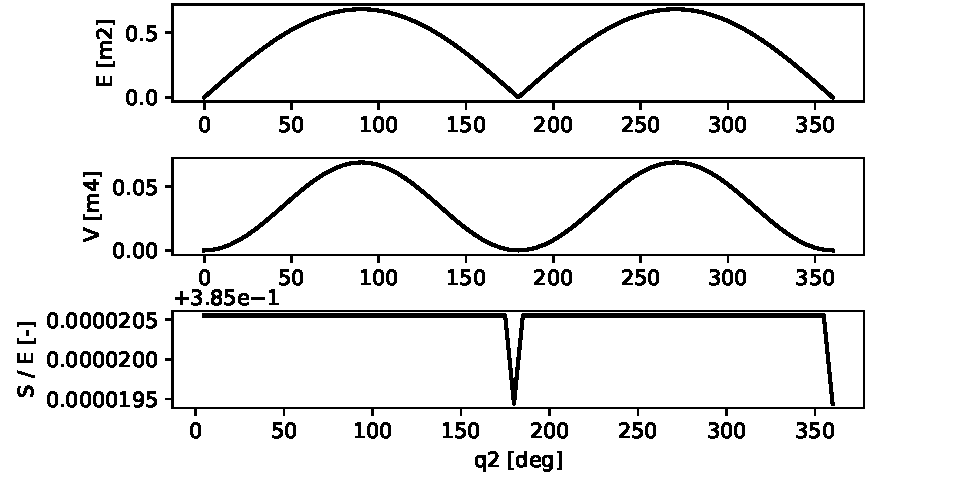
\includegraphics[width=80truemm]{./simulation/length_plots.pdf}
  \caption{(I)の場合における拡張可操作度の期待値、分散、標準偏差/期待値}
  \label{fig:case_i}
  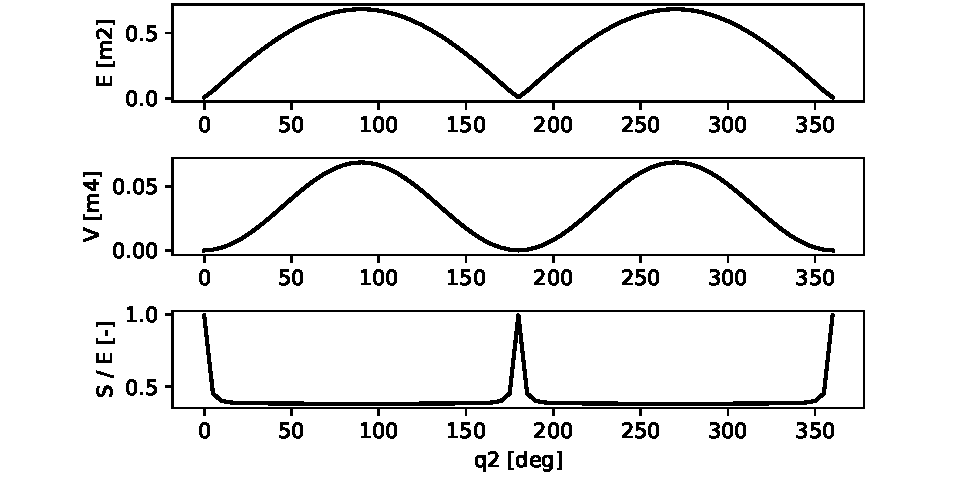
\includegraphics[width=80truemm]{./simulation/angle_plots.pdf}
  \caption{(II)の場合における拡張可操作度の期待値、分散、標準偏差/期待値}
  \label{fig:case_ii}
\end{figure}
標準偏差/期待値にわずかな差異が生じているが、その他の変化ほとんど確認することができなかった。

\end{document}
